\documentclass[twocolumn,a4j]{jsarticle}
\setlength{\topmargin}{-20.4cm}
\setlength{\oddsidemargin}{-10.4mm}
\setlength{\evensidemargin}{-10.4mm}
\setlength{\textwidth}{18cm}
\setlength{\textheight}{26cm}

\usepackage[top=13truemm,bottom=20truemm,left=15truemm,right=15truemm]{geometry}
\usepackage[latin1]{inputenc}
\usepackage{amsmath}
\usepackage{amsfonts}
\usepackage{amssymb}
\usepackage[dvipdfmx]{graphicx}
\usepackage[dvipdfmx]{color}
\usepackage{listings}
\usepackage{listings,jvlisting}
\usepackage{geometry}
\usepackage{framed}
\usepackage{color}
\usepackage[dvipdfmx]{hyperref}
\usepackage{ascmac}
\usepackage{enumerate}
\usepackage{tabularx}
\usepackage{cancel}
\usepackage{scalefnt}

\renewcommand{\figurename}{Fig.}
\renewcommand{\tablename}{Table }

\lstset{
basicstyle={\ttfamily},
identifierstyle={\small},
commentstyle={\smallitshape},
keywordstyle={\small\bfseries},
ndkeywordstyle={\small},
stringstyle={\small\ttfamily},
frame={tb},
breaklines=true,
columns=[l]{fullflexible},
xrightmargin=0zw,
xleftmargin=3zw,
numberstyle={\scriptsize},
stepnumber=1,
numbersep=1zw,
lineskip=-0.5ex
}

\makeatletter
\def\@maketitle
{
\begin{center}
{\LARGE \@title \par}
\end{center}
\begin{flushright}
{\large \@date}\\
{\large{京都工芸繊維大学 工芸科学部 機械工学課程}}\\
{\large \@author}
\end{flushright}
\par\vskip 1.5em
}
\makeatother

\setcounter{tocdepth}{3}

\author{来代 勝胤 / Masatsugu KITADAI}
\title{令和3年度 1月度 報告書}
\date{2022/1/23}

\begin{document}
\columnseprule=0.1mm

\maketitle
\section*{報告内容}
\begin{enumerate}[1.]
    \item 進捗状況
    \item 実験装置の製作
    \item 実験の実施と結果
    \item 補正理論と適用結果
    \item 今月の進捗と今後の予定
\end{enumerate}

\section{進捗状況}
今月は,12月に行った模擬実験方法を基準に自動ステージを用いて
製作した実験装置を使用して性能評価実験を行った.
また,実験結果に対しての補正理論を作成し,それを用いてデータ処理を行った.

\section{実験装置の製作}

前回の模擬実験では,人為的操作を含む実験を行ったが,
再現性が保証できないことや実験を複数回行うことが困難であることから
自動一軸ステージ,自動回転ステージを用いて実験を自動化し,
\textgt{可能な限りの人為的操作を削除すること,実験回数の確保すること}
を目標に新たに実験装置を製作した.
以下のFig.に実験装置の3Dモデル,Fig.に製作した実験装置の写真を示す.

\begin{figure}[htbp]
    \footnotesize
    \begin{center}
        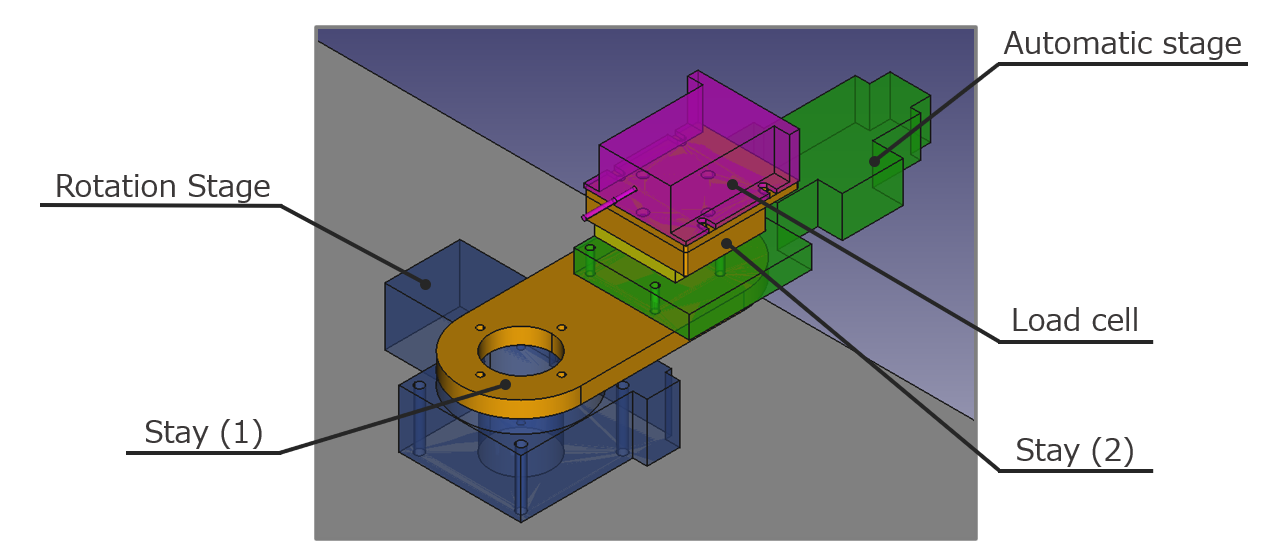
\includegraphics[width=85mm]{../images/21-1.png}
        \caption{Automatic experimental device (3D CAD)}
        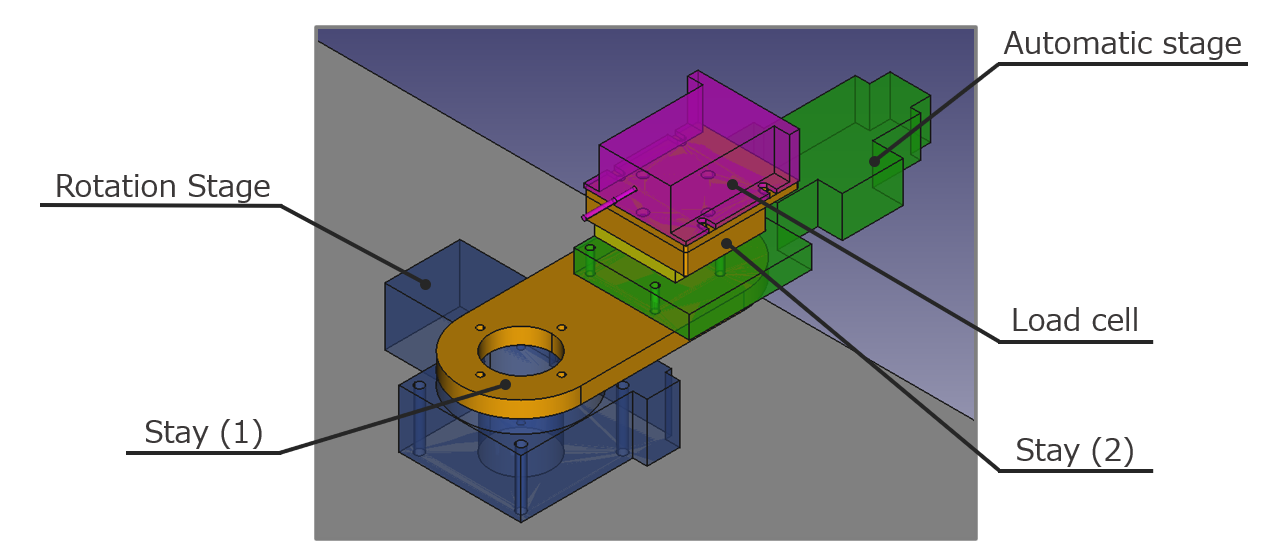
\includegraphics[width=85mm]{../images/21-1.png}
        \caption{Automatic experimental device (Photo)}
    \end{center}
\end{figure}

\newpage

\section{実験の実施と結果}

\subsection{実験条件}

今回の実験は以下の条件で行った.
また,実験の測定準備・測定手順においては前回の模擬実験と同様である.

\begin{table}[htbp]
    \begin{center}
        \begin{tabular}{|p{30mm}|p{20mm}|p{30}|}
            \hline
            \multicolumn{1}{|c|}{\textgt{項目}} & \multicolumn{1}{|c|}{\textgt{条件数}} & \multicolumn{1}{|c|}{\textgt{備考}}\\ \hline
            \multicolumn{1}{|c|}{測定角度}                    & \multicolumn{1}{|c|}{24} & \multicolumn{1}{|c|}{\textgt{15度ごとの測定}}  \\ \hline
            \multicolumn{1}{|c|}{試行回数}                    & \multicolumn{1}{|c|}{5} & \multicolumn{1}{|c|}{\textgt{}}  \\ \hline
        \end{tabular}
    \end{center}
\end{table}

\subsection{実験結果}
今回の実験結果について以下のFig.~Fig.に示す.
なお,ここでは実験1回目における 0 [deg],45 [deg]についての結果を示している.

\begin{figure}[htbp]
    \footnotesize
    \begin{center}
        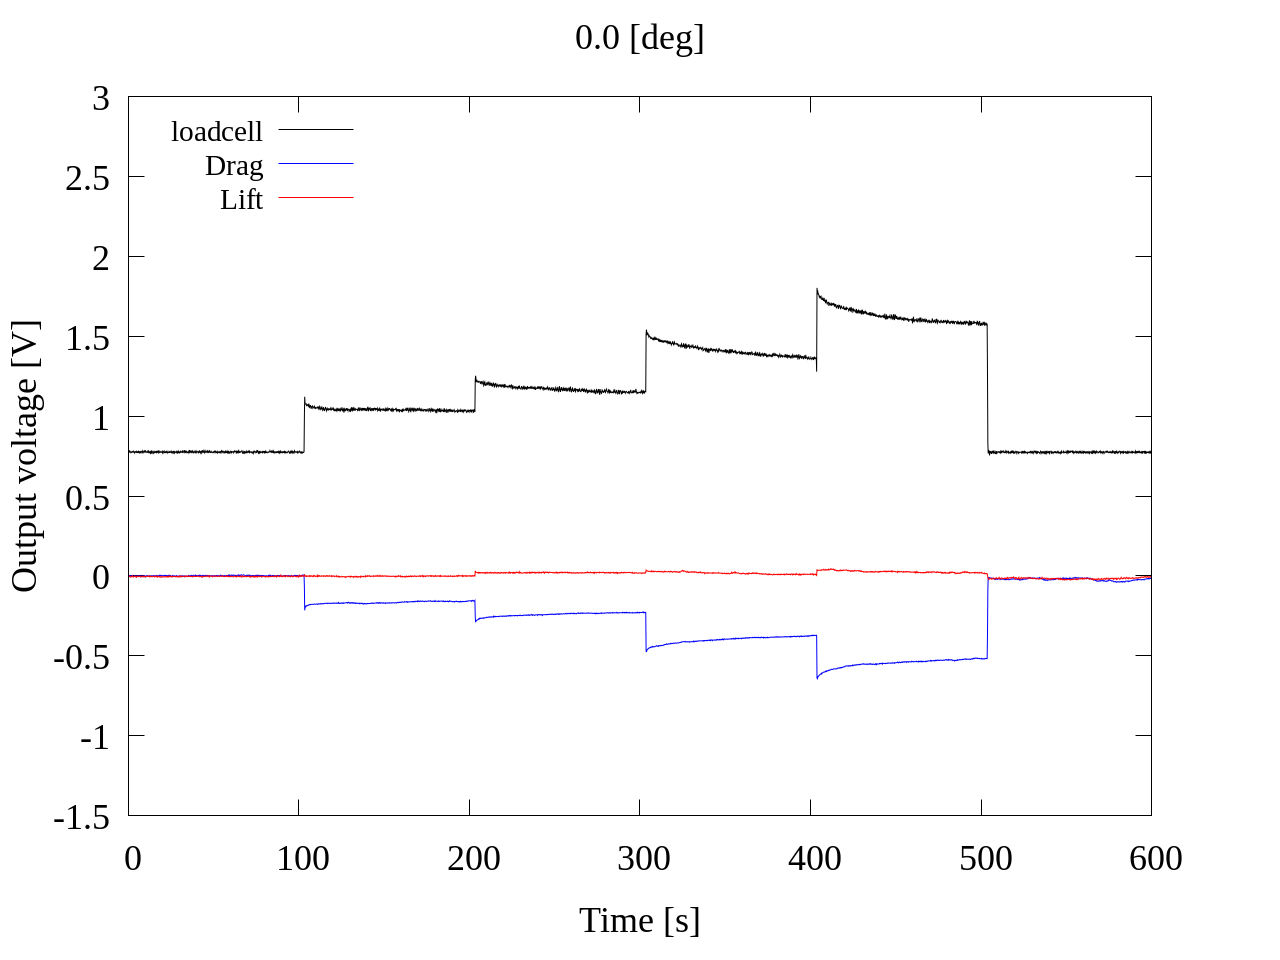
\includegraphics[width=82mm]{../../../02_workspace/result/2-1/plot/01-3_allsensors/01_allsensors_0.png}
        \caption{Output voltage (0 [deg])}
        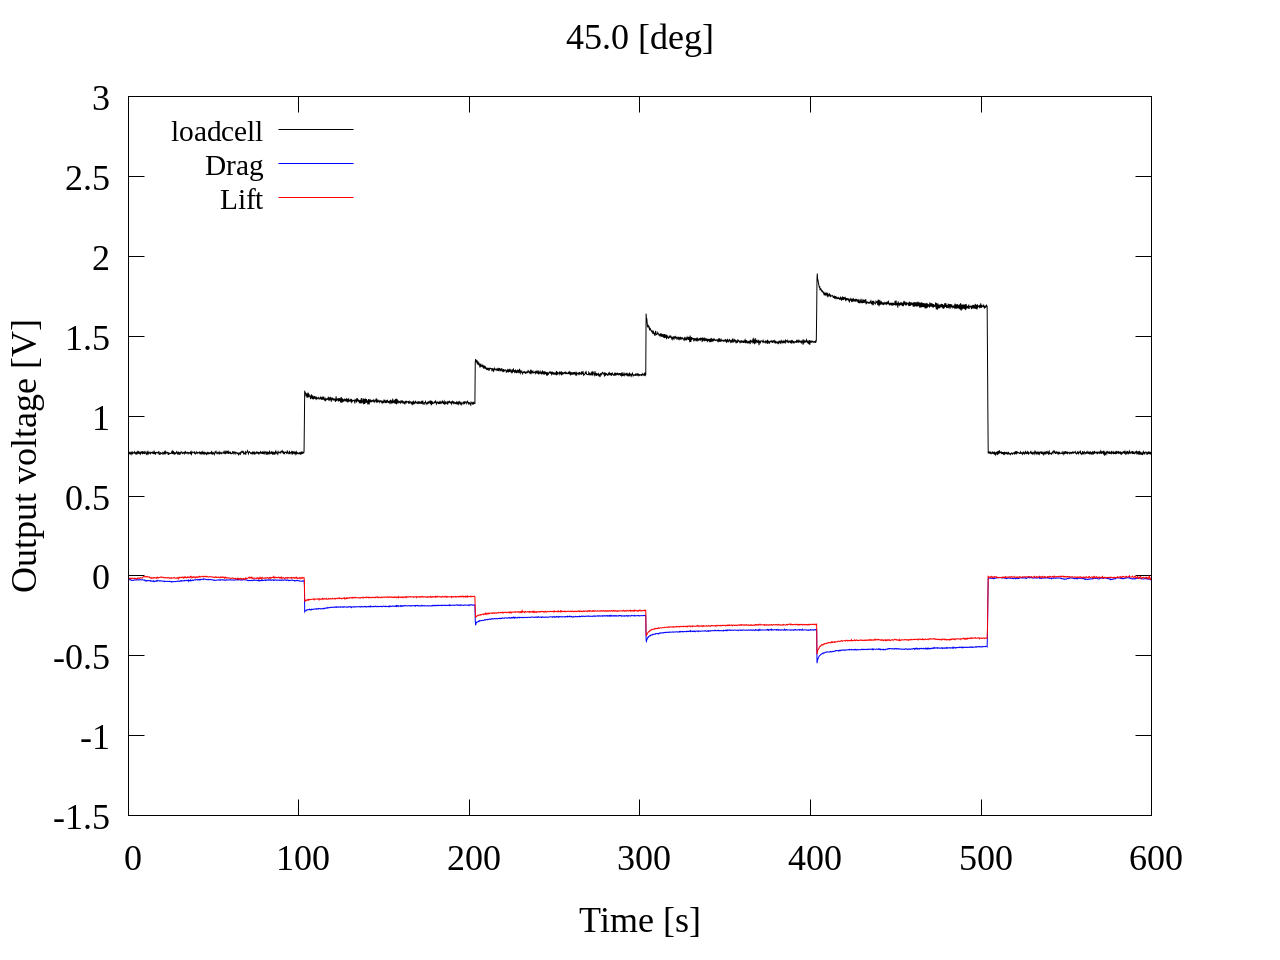
\includegraphics[width=82mm]{../../../02_workspace/result/2-1/plot/01-3_allsensors/01_allsensors_450.png}
        \caption{Output voltage (45 [deg])}
    \end{center}
\end{figure}

\newpage
Fig.4,Fig.5より,自動ステージを用いることによってノイズが除去されていることがわかる.
また,自動一軸ステージが移動した直後から出力電圧の減衰が見られる場合があるが,
同様の変化がロードセルおよびひずみセンサにみられることから大きな問題ではないと考える.\\

\subsection{出力電圧勾配による評価}

実験結果の処理手順に沿って出力電圧勾配を算出する.
1~5回目の実験結果について,以下のFig.5~Fig.9に示す.

\begin{figure}[htbp]
    \footnotesize
    \begin{center}
        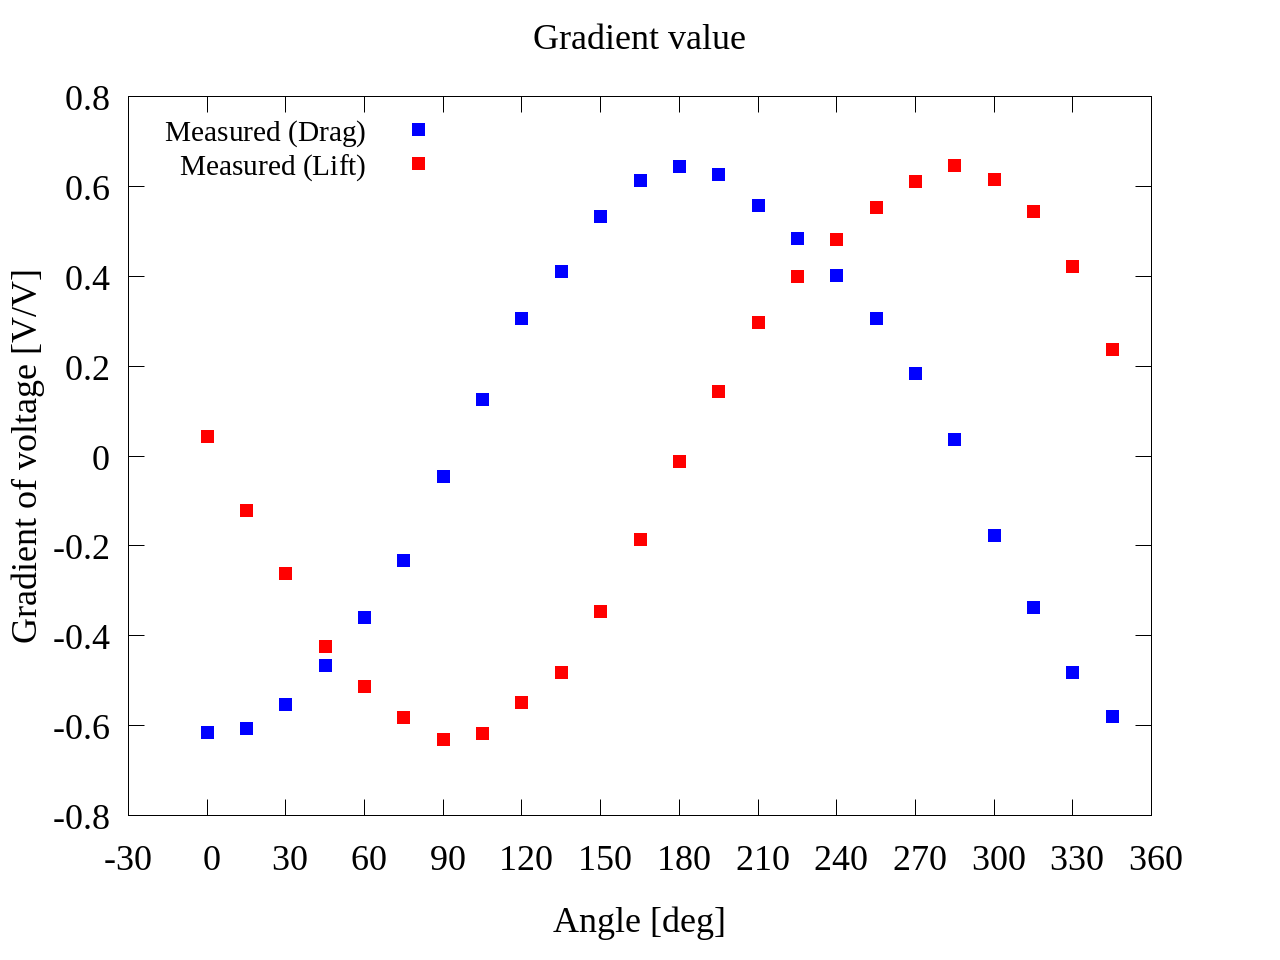
\includegraphics[width=80mm]{../../../02_workspace/result/2-1/plot/05/05_summary-wave.png}
        \caption{Gradient of output voltage (1st)}
        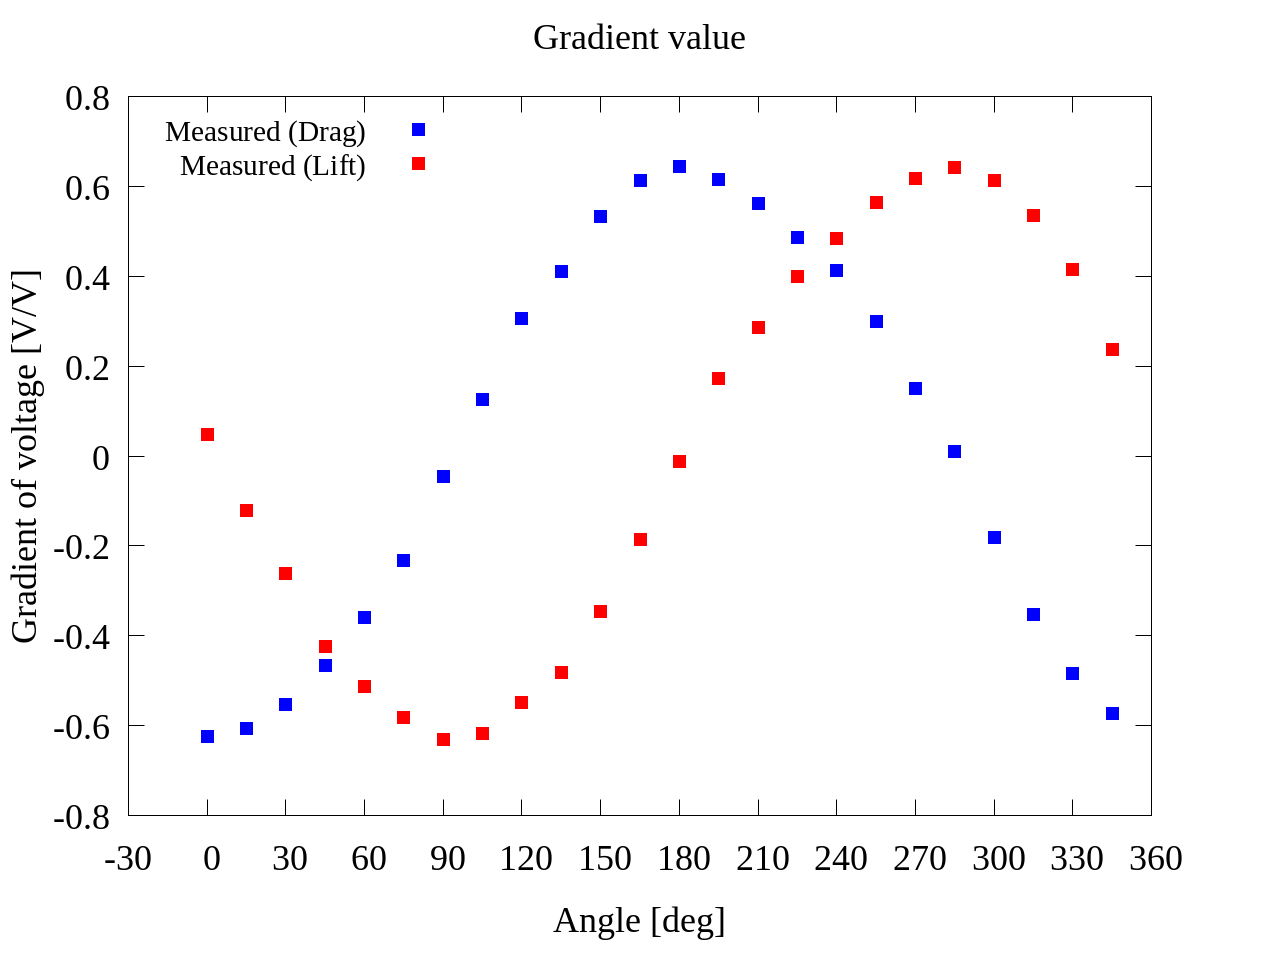
\includegraphics[width=80mm]{../../../02_workspace/result/2-2/plot/05/05_summary-wave.png}
        \caption{Gradient of output voltage (2nd)}
        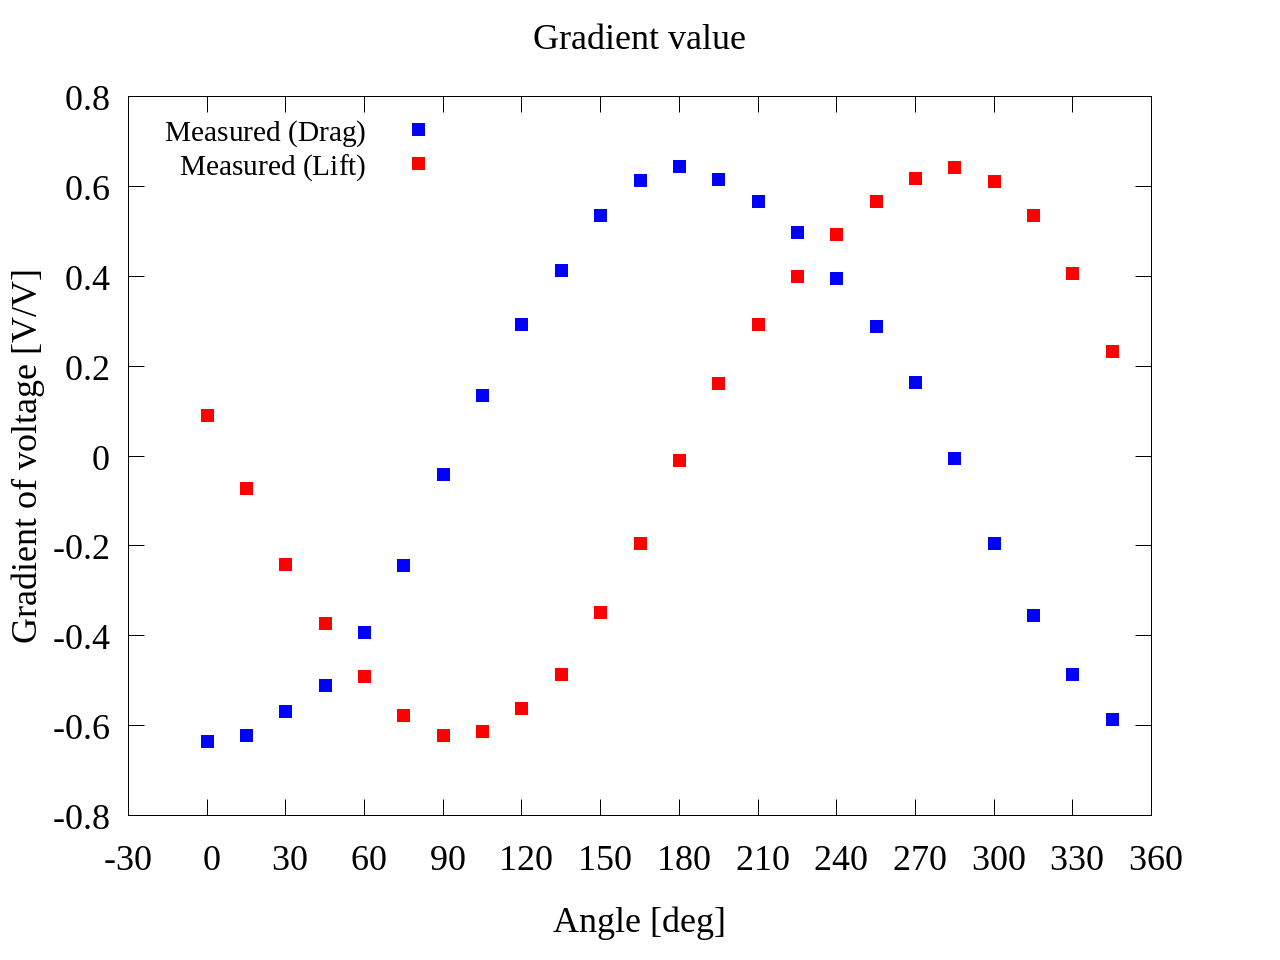
\includegraphics[width=80mm]{../../../02_workspace/result/2-3/plot/05/05_summary-wave.png}
        \caption{Gradient of output voltage (3rd)}
    \end{center}
\end{figure}

\begin{figure}[htbp]
    \footnotesize
    \begin{center}
        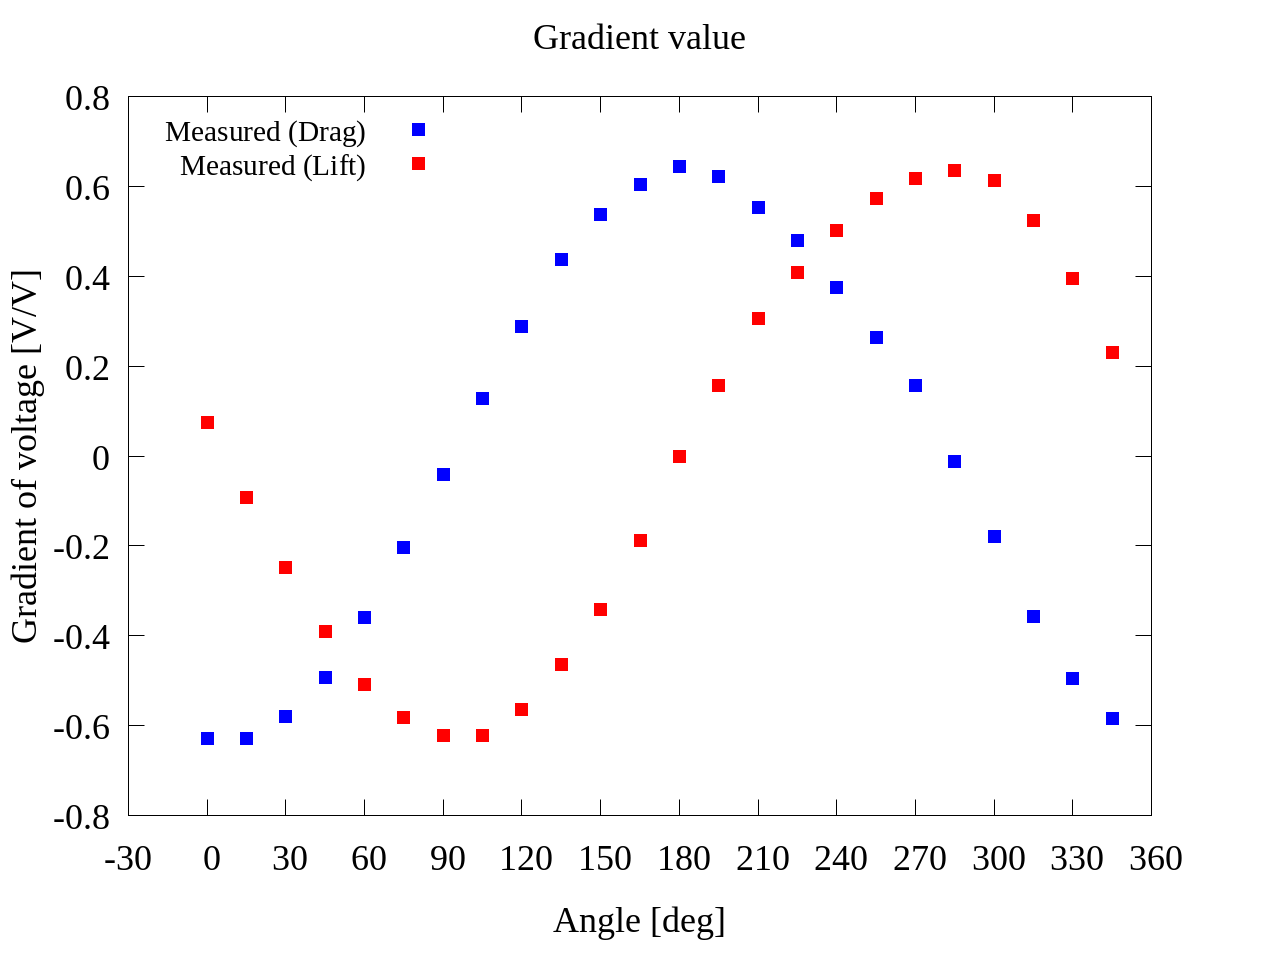
\includegraphics[width=80mm]{../../../02_workspace/result/2-4/plot/05/05_summary-wave.png}
        \caption{Gradient of output voltage (4th)}
        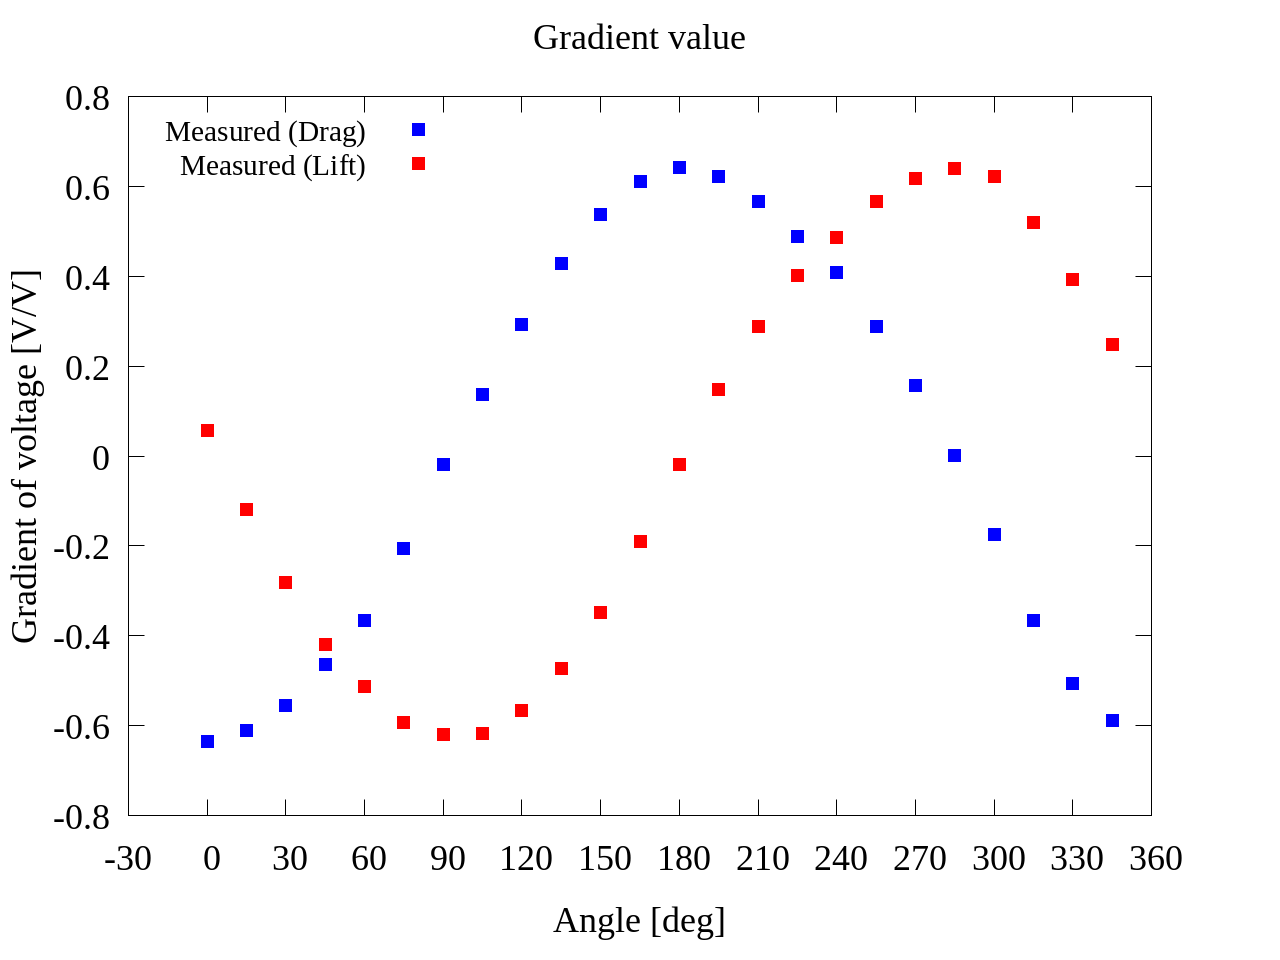
\includegraphics[width=80mm]{../../../02_workspace/result/2-5/plot/05/05_summary-wave.png}
        \caption{Gradient of output voltage (5th)}
    \end{center}
\end{figure}

出力電圧勾配に対する補正処理ついては実験結果の一般性を保証するため
計5回の実験結果の平均値を用いることとする.
その平均値を示した図をFig.10に示す.

\begin{figure}[htbp]
    \footnotesize
    \begin{center}
        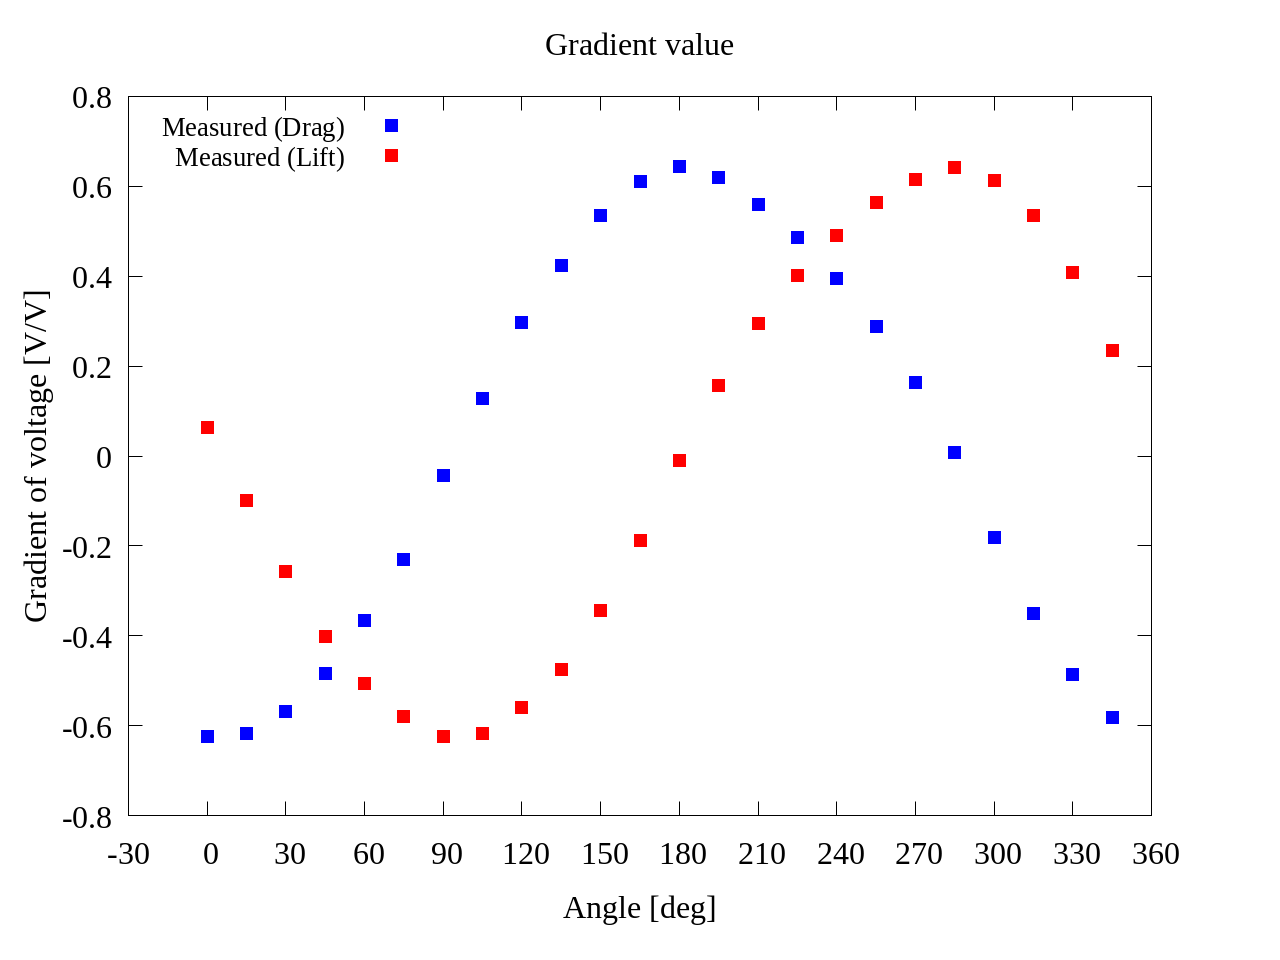
\includegraphics[width=80mm]{../../../02_workspace/result/2-ex/plot/05/05_summary-wave.png}
        \caption{Gradient of output voltage (Average)}
    \end{center}
\end{figure}

また,それそれの角度の値について
抗力方向の出力電圧勾配を$v_d$,揚力方向を$v_l$として次ページのTable 1に示す.

\begin{table}[htbp]
    \begin{center}
        \caption{Result summary}
        \begin{tabular}{|p{20mm}|p{20mm}|p{20mm}|}
            \hline
            \multicolumn{1}{|c|}{\textgt{Angle [deg]}} & \multicolumn{1}{|c|}{\textgt{$v_d$ [V/V]}} & \multicolumn{1}{|c|}{\textgt{$v_l$ [V/V]}} \\ \hline
            \multicolumn{1}{|c|}{0}                  & \multicolumn{1}{|r|}{-0.627}           & \multicolumn{1}{|r|}{ 0.063} \\ \hline
            \multicolumn{1}{|c|}{15}                 & \multicolumn{1}{|r|}{-0.617}           & \multicolumn{1}{|r|}{-0.103}  \\ \hline
            \multicolumn{1}{|c|}{30}                 & \multicolumn{1}{|r|}{-0.566}           & \multicolumn{1}{|r|}{-0.261}  \\ \hline
            \multicolumn{1}{|c|}{45}                 & \multicolumn{1}{|r|}{-0.479}           & \multicolumn{1}{|r|}{-0.405}  \\ \hline
            \multicolumn{1}{|c|}{60}                 & \multicolumn{1}{|r|}{-0.365}           & \multicolumn{1}{|r|}{-0.508}  \\ \hline
            \multicolumn{1}{|c|}{75}                 & \multicolumn{1}{|r|}{-0.226}           & \multicolumn{1}{|r|}{-0.582}  \\ \hline
            \multicolumn{1}{|c|}{90}                 & \multicolumn{1}{|r|}{-0.038}           & \multicolumn{1}{|r|}{-0.624}  \\ \hline
            \multicolumn{1}{|c|}{105}                & \multicolumn{1}{|r|}{0.131}            & \multicolumn{1}{|r|}{-0.618}  \\ \hline
            \multicolumn{1}{|c|}{120}                & \multicolumn{1}{|r|}{0.296}            & \multicolumn{1}{|r|}{-0.560}  \\ \hline
            \multicolumn{1}{|c|}{135}                & \multicolumn{1}{|r|}{0.425}            & \multicolumn{1}{|r|}{-0.474} \\ \hline
            \multicolumn{1}{|c|}{150}                & \multicolumn{1}{|r|}{0.536}            & \multicolumn{1}{|r|}{-0.345} \\ \hline
            \multicolumn{1}{|c|}{165}                & \multicolumn{1}{|r|}{0.611}            & \multicolumn{1}{|r|}{-0.189} \\ \hline
            \multicolumn{1}{|c|}{180}                & \multicolumn{1}{|r|}{0.643}            & \multicolumn{1}{|r|}{-0.011} \\ \hline
            \multicolumn{1}{|c|}{195}                & \multicolumn{1}{|r|}{0.620}            & \multicolumn{1}{|r|}{0.156} \\ \hline
            \multicolumn{1}{|c|}{210}                & \multicolumn{1}{|r|}{0.561}            & \multicolumn{1}{|r|}{0.294} \\ \hline
            \multicolumn{1}{|c|}{225}                & \multicolumn{1}{|r|}{0.487}            & \multicolumn{1}{|r|}{0.402} \\ \hline
            \multicolumn{1}{|c|}{240}                & \multicolumn{1}{|r|}{0.399}            & \multicolumn{1}{|r|}{0.489} \\ \hline
            \multicolumn{1}{|c|}{255}                & \multicolumn{1}{|r|}{0.289}            & \multicolumn{1}{|r|}{0.565} \\ \hline
            \multicolumn{1}{|c|}{270}                & \multicolumn{1}{|r|}{0.163}            & \multicolumn{1}{|r|}{0.616} \\ \hline
            \multicolumn{1}{|c|}{285}                & \multicolumn{1}{|r|}{0.006}            & \multicolumn{1}{|r|}{0.641} \\ \hline
            \multicolumn{1}{|c|}{300}                & \multicolumn{1}{|r|}{-0.181}           & \multicolumn{1}{|r|}{0.615} \\ \hline
            \multicolumn{1}{|c|}{315}                & \multicolumn{1}{|r|}{-0.353}           & \multicolumn{1}{|r|}{0.532} \\ \hline
            \multicolumn{1}{|c|}{330}                & \multicolumn{1}{|r|}{-0.490}           & \multicolumn{1}{|r|}{0.406} \\ \hline
            \multicolumn{1}{|c|}{345}                & \multicolumn{1}{|r|}{-0.582}           & \multicolumn{1}{|r|}{0.237} \\ \hline
        \end{tabular}
    \end{center}
\end{table}

\newpage

\section{補正理論と適用結果}

作用力測定装置から得た抗力方向および揚力方向における出力電圧$V_D$,$V_L$を
正規座標系の$x$軸方向および$y$軸方向の荷重$F_x$,$F_y$に換算する際に,
出力電圧$V_D$,$V_L$と$F_x$,$F_y$の関係性を明らかにするための校正実験を
行う必要がある.\\

\subsection{作用力測定装置と校正実験装置の関係}
作用力測定装置と校正実験装置の設置位置によって校正実験結果は大きく変動するため,
その影響を考慮し,補正処理を行う必要がある.
このとき以下のような要因が,校正実験結果への影響を与えていると考えられる.

\begin{enumerate}[(1)]
    \item 作用力測定装置のひずみセンサの取付
    \item 作用力測定装置の回流水槽への設置
    \item 作用力測定装置と校正装置の設置
\end{enumerate}

\newpage

ここで,水流に対する座標系を正規座標系 $(x,y)$,
作用力測定装置の座標系を座標系(1) $(x',y')$,
校正装置の座標系を座標系(2) $(x,'' y'')$とする.

このとき,(1) 作用力測定装置のひずみセンサの取付,
(2) 作用力測定装置の回流水槽への取付 の際に正確に取り付けられていることを保証できないことから
座標系[1]は正規座標系に対して
$x'$軸は$x$軸から$\theta_x$,$y'$軸は$y$軸から$\theta_y$だけ回転している.
また,座標系[2]は正規座標系に対して
$x''$軸は$x$軸から$y$方向に$\Delta x$,
$y''$軸は$y$軸から$x$方向に$\Delta y$だけオフセットを持つ状態となると考えられる.

\begin{figure}[htbp]
    \footnotesize
    \begin{center}
        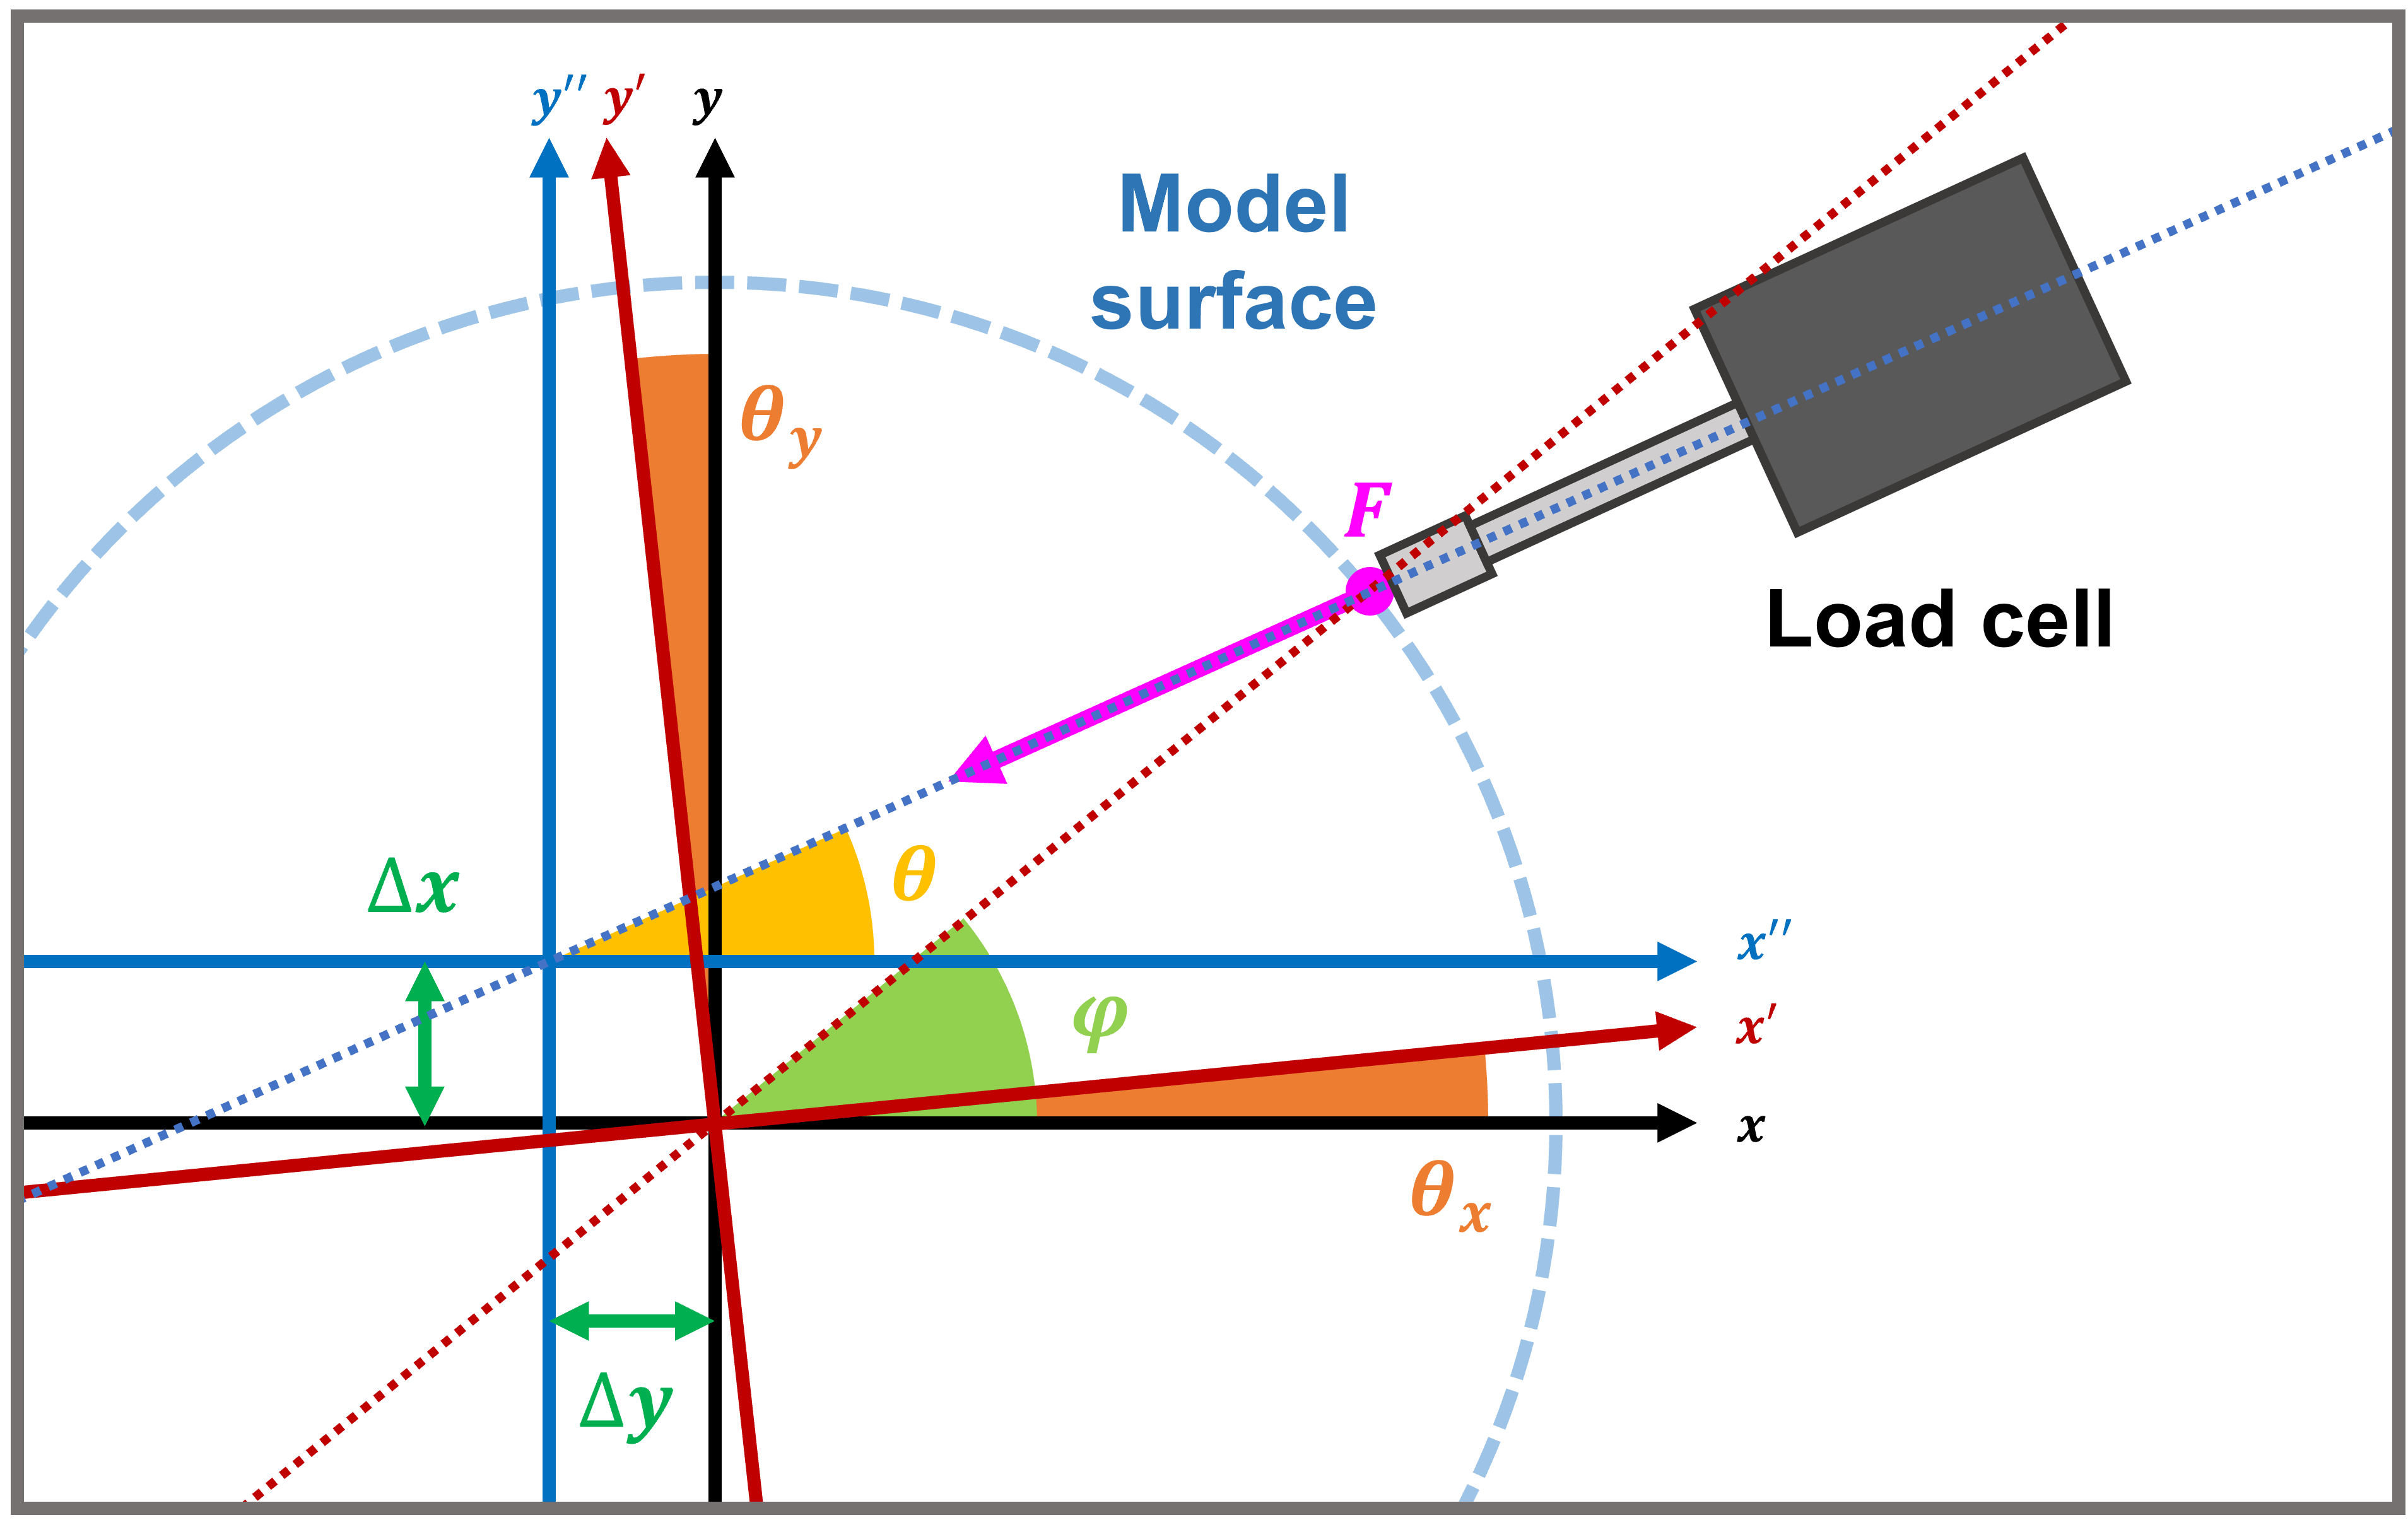
\includegraphics[width=80mm]{../images/31-1.png}
        \caption{}
    \end{center}
\end{figure}

\section{今月のまとめと今後の予定}
\begin{itemize}
    \item [$\blacksquare$] 今月のまとめ
          \begin{itemize}
              \item [$\bullet$] 製作した実験装置を用いて性能評価実験を行った
              \item [$\bullet$] 自動化することで,人為的操作による非再現性を取り除き,
                                実験回数を大幅に向上することができた
              \item [$\bullet$] 実験結果の補正理論を作成しデータ処理を行った
              \item [$\bullet$] テストデータへの補正理論適用結果から
                                おおよそ問題がないことが確認できた
              \item [$\bullet$] 2ゲージ法による影響を考慮する必要があることがわかった.
          \end{itemize}
          \vskip\baselineskip
    \item [$\blacksquare$] 2月の予定
          \begin{itemize}
              \item [$\bullet$] 卒業論文の執筆
              \item [$\bullet$] 実験の実施 (1月末まで)
              \item [$\bullet$] 新たな補正方法の検討
          \end{itemize}
\end{itemize}
\end{document}